\section{Nested-Word Automata and Overview of the Library's Organization}
\label{Se:Nested Word Automata}

WALi-NWA is a library for constructing, querying, and operating on nested-word automata.  It
is implemented in C++.

\subsection{Nested Words and Nested-Word Automata}
\label{Se:Def}

Nested-word automata (NWAs)~\cite{DLT:AM2006,JACM:AM09} are a generalization
of finite-state automata that can capture the matched-parenthesis structure
that is exibited by, for example, opening and closing tags in XML and the
call/return structure exhibited by execution traces in multi-procedure
programs. Their languages represent somewhat of a middle-ground between
standard regular languages and context-free languages. Nested-word languages
retain the call/return structure mentioned above, which makes them a
refinement of standard regular languages. For instance, there is an NWA that
accepts exactly the language of properly-balanced parentheses (with the
associated matching structure). However, they also retain all the closure
properties that makes standard regular languages attractive; in particular,
they are closed under complementation and intersection. However, they are not
directly comparable to languages of linear words, as the call/return
structure is an explicit part of each word of a nested-word language.

\begin{definition}
  A \textsl{nested word} $(w,\rightsquigarrow)$ over alphabet $\Sigma$ is an
  ordinary (linear) word $w \in \Sigma^*$ of length $|w|$ together with a
  \textsl{nesting relation} $\rightsquigarrow$.

  The relation $\rightsquigarrow$ is a collection of edges (over the
  positions in $w$) that do not cross. Formally, $\rightsquigarrow \subseteq$
  $\{-\infty, 1, 2, \ldots, |w| \} \times \{1, 2, \ldots, |w|, +\infty\}$
  such that:
  \begin{itemize}
    \item
      Nesting edges only go forward: if $i \rightsquigarrow j$ then $i < j$.
    \item
      No two edges share a position: for $1 \leq i \leq |w|$, there is at
      most one $j$ such that $i \rightsquigarrow j$ or $j \rightsquigarrow
      i$.
    \item
      Edges do not cross: if $i \rightsquigarrow j$ and $i' \rightsquigarrow
      j'$, then one cannot have $i < i' \leq j < j'$.
  \end{itemize}

  When $i \rightsquigarrow j$ holds, for $1 \leq i \leq |w|$, $i$ is called a
  \textsl{call} position. If $i \rightsquigarrow +\infty$, then $i$ is a
  \textsl{pending call}; otherwise $i$ is a \textsl{matched call}, and the
  (unique) position $j$ such that $i \rightsquigarrow j$ is called its
  \textsl{return successor}. (Note that these terms refer to positions within
  $w$ rather than the symbol.)

  Similarly, when $i \rightsquigarrow j$ holds, for $1 \leq j \leq |w|$, $j$
  is a \textsl{return} position. If $-\infty \rightsquigarrow j$, then $j$ is
  a \textsl{pending return}, otherwise $j$ is a \textsl{matched return}, and
  the (unique) position $i$ such that $i \rightsquigarrow j$ is called its
  \textsl{call predecessor}.

  A position $1 \leq i \leq |w|$ that is neither a call nor a return is an
  \textsl{internal} position.

  A nested word is \textsl{balanced} if it has no pending calls
  or returns.  A nested word is \textsl{unbalanced-left} (or a
  \textsl{nested-word prefix}) if it has pending returns, and it is
  \textsl{unbalanced-right} (or a \textsl{nested-word suffix})
  if it has no pending calls.

\end{definition}

\TODO{Uh, what does this mean?}
The library supports unbalanced-left, unbalanced-right, and balanced
nested words, but has no direct support for general nested words.  For the
effects of boolean operations on the four kinds of nested-words see Figure
\ref{Fig:Ops}.

\begin{figure}[htb]
  \centering
\begin{tabular}{c@{\hspace{1cm}}c}
  \begin{tabular}{|| r || l | l | l | l ||}
\hhline{|t:=====:t|}
    Intersection & B & UL & UR & NW \\
\hhline{||=#=|=|=|=||}
    B & B & B & B & B \\
\hhline{||-||-|-|-|-||}
    UL & B & UL & B & UL \\
 \hhline{||-||-|-|-|-||}
    UR & B & B & UR & UR \\
\hhline{||-||-|-|-|-||}
    NW & B & UL & UR & NW \\
\hhline{|b:=====:b|}
  \end{tabular}
\vspace{1cm} &
  \begin{tabular}{|| r || l | l | l | l ||}
\hhline{|t:=====:t|}
    Concatenation & B & UL & UR & NW \\
\hhline{||=#=|=|=|=||}
    B & B & UL & UR & NW \\
\hhline{||-||-|-|-|-||}
    UL & UL & UL & NW & NW \\
\hhline{||-||-|-|-|-||}
    UR & UR & NW & UR & NW \\
\hhline{||-||-|-|-|-||}
    NW & NW & NW & NW & NW \\
\hhline{|b:=====:b|}
  \end{tabular} \\
\vspace{1cm}
  \begin{tabular}{|| r || l | l | l | l ||}
\hhline{|t:=====:t|}
    Union & B & UL & UR & NW \\
\hhline{||=#=|=|=|=||}
    B & B & UL & UR & NW \\
\hhline{||-||-|-|-|-||}
    UL & UL & UL & NW & NW \\
\hhline{||-||-|-|-|-||}
    UR & UR & NW & UR & NW \\
\hhline{||-||-|-|-|-||}
    NW & NW & NW & NW & NW \\
\hhline{|b:=====:b|}
  \end{tabular} &
  \begin{tabular}{|| r || l | l | l | l ||}
\hhline{|t:=====:t|}
    Operation & B & UL & UR & NW \\
\hhline{||=#=|=|=|=||}
    Star & B & UL & UR & NW \\
\hhline{||-||-|-|-|-||}
    Reverse & B & UR & UL & NW \\
\hhline{||-||-|-|-|-||}
    Complement & UL & UL & UR & NW \\
\hhline{|b:=====:b|}
  \end{tabular} \\
\end{tabular}
  \caption{Table of Operations on Nested Words. Note: B = balanced nested-word, UR = unbalanced-right nested-word, UL = unbalanced-left nested-word, NW = nested-word}
  \label{Fig:Ops}
\end{figure}


\begin{definition}
  \label{De:NWA}

  A \textsl{nested-word language} is any set of nested words; such a language
  is a \textsl{regular nested-word language} if it is accepted by a NWA as
  defined below.


  A \textsl{nested-word automaton} (NWA) $A$ is a 5-tuple $(Q, \Sigma, Q_0,
  \delta, F)$, where $Q$ is a finite set of states, $\Sigma$ is a finite
  alphabet, $Q_0 \subseteq Q$ is the initial state, $F \subseteq Q$ is a set of
  final states, and $\delta$ is a transition relation. The transition
  relation $\delta$ consists of three components, $(\delta_c, \delta_i,
  \delta_r)$, where:
  \begin{itemize}
    \item
      $\delta_i: (Q \times \Sigma) \times Q$ is the transition relation for
      internal positions of the input word.
    \item
      $\delta_c: (Q \times \Sigma) \times Q$ is the transition relation for
      call positions.
    \item
      $\delta_r: (Q \times Q \times \Sigma) \times Q$ is the transition
      relation for return positions.
  \end{itemize}

  Starting from a state in $Q_0$, an NWA $A$ reads a nested word $(w,\rightsquigarrow)$
  from left to right, and performs transitions according to the current input
  symbol and $\rightsquigarrow$.  If $A$ is in state $q$ when reading input
  symbol $\sigma$ at position $i$ in $w$, and $i$ is an internal (resp, call)
  position in $\rightsquigarrow$, $A$ makes a transition to a state $q'$ (if
  one is available) such that $(q,\sigma,q')\in\delta_i$ (resp,
  $(q,\sigma,q')\in\delta_c$).  If $i$ is a return position, let $k$ be the
  call predecessor of $i$ (so $k \rightsquigarrow i$) and $q_c$ be the state
  $A$ was in just before the transition it made on the $k^{\textrm{th}}$
  symbol; $A$ changes to a state $q'$ such that $(q,q_c,\sigma,q')
  \in\delta_r$. If there is a computation of $A$ on input
  $(w,\rightsquigarrow)$ that terminates in a state $q\in F$, then $A$
  accepts $(w,\rightsquigarrow)$.

  NWAs can be either deterministic or nondeterministic, and these types have
  equivalent power.
\end{definition}


To distinguish among the different roles for states in an internal
transition $(q,\sigma,q')$, we say that $q$ is the source and $q'$ is the
target.  Similarly, to distinguish among the roles for states in a call
transition $(q_c,\sigma,q_e)$, we say that $q_c$ is the call state and $q_e$
is the entry state. To distinguish among the roles for states in a return
transition $(q_x,q_c,\sigma,q_r)$, we say that $q_x$ is the exit state,
$q_c$ is the call state (or call predecessor), and $q_r$ is the return state.


\subsection{Classes}
\label{Se:Classes}

\begin{description}

\item NWA \nopagebreak

  Models nested-word automata.  This is the main class of the WALi-NWA package.

\item NestedWord \nopagebreak

  This class models a single nested word. (It can be balanced or unbalanced.)

\item ClientInfo \nopagebreak

  Additional information that can be attached to NWA states. Clients of the
  NWA library can subclass ClientInfo and attach instances to states in the
  automaton.

\item WeightGen \nopagebreak

  Weight-generation algorithms for the NWA to WPDS conversion and prestar and
  poststar reachability queries.

\item Key \nopagebreak

  This is a unique idenitifier for states and symbols in an NWA or
  NestedWord; it is actually a typedef of an integer, though client code
  should not depend on this fact. See \cite{wali}.

\item WPDS \nopagebreak

  Models weighted pushdown systems.  See \cite{wali}.

\item WFA \nopagebreak

  Models weighted finite automata.  See \cite{wali}.

\item ref\_ptr$<$T$>$ \nopagebreak

  An (intrusive) reference-counting smart pointer template.  See \cite{wali}.
  WALi-NWA provides a typedef of ref\_ptr$<$NWA$>$ called NWARefPtr. Several
  functions in the library's interface use this typedef.

\end{description}


\subsection{Construction}
\label{Se:Construction}

The NWA provides two constructors, the default constructor and the copy
constructor. The default constructor creates an empty NWA. Thereafter, 
client code can \begin{inparaenum} \item add or remove states, \item add or remove
symbols, \item add or remove transitions, \item set the status of certain
  states as initial or final, and \item combine component NWAs (via union,
  intersection, etc). \end{inparaenum}


The following functions are related to construction:
\begin{description}
  \item \texttt{NWA::NWA()}) constructs an empty NWA

  \item \texttt{NWA::NWA(NWA const \& other)} Copies \texttt{other}; the
    automata will not share structure

  \item \texttt{NWA::operator=(NWA const \& other)} Assigns \texttt{other} to \texttt{this};
    the automata will not share structure.

  \item \texttt{NWA::clear()} \nopagebreak
    Removes all states, symbols, and transitions from the NWA.

\end{description}



\subsection{Examples}
\label{Se:Examples}

As an example, consider the nested word automaton $A = (Q_A, \Sigma_A,
{Q_0}_A, \delta_A, F_A)$ where $Q_A = \{Start, Call, Entry, State, Exit,
Return, End\}$, $\Sigma_A = \{a,
call, b, ret\}$, ${Q_0}_A = \{Start\}$, $F_A = \{End\}$, and \\
$\delta_A = 
\begin{cases} 
\delta_i = \{(Start,a,Call), (Entry,b,State), (State,b,Exit), (Return,a,End)\}, \\
\delta_c = \{(Call,call,Entry)\}, \\ 
\delta_r = \{(Exit,Call,ret,Return)\}, \\ 
\end{cases}$ \\
as seen in Figure \ref{Fig:Example1}.
 
\begin{figure}[htb]
  \centering
    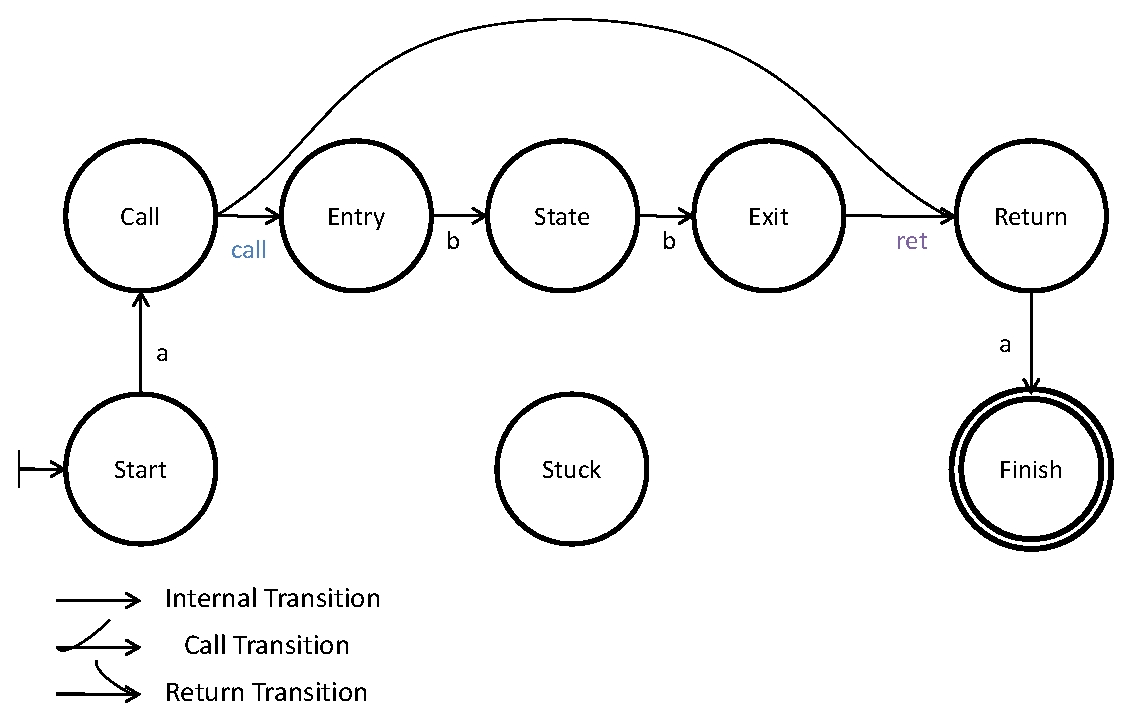
\includegraphics[width=12cm]{Figures/Figure1}
  \caption{An example NWA.}
  \label{Fig:Example1}
\end{figure}

